Для установки всего необходимого, нам нужно открыть терминал, нажав на его иконку. 

\begin{figure}[h]
		\centering
		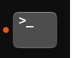
\includegraphics[width=0.2\linewidth]{VM/5.png}
\caption{Терминал.}
\label{ris:image}
\end{figure}

Далее, для скачивания, необходимо ввести соответствующие команды:
\newline git – \texttt{sudo apt install git}
\newline nodejs – \texttt{sudo apt install nodejs}
\newline npm - \texttt{sudo apt install npm}
\newline grunt - \texttt{sudo apt install grunt}
\newline Чтобы удостовериться, что всё правильно скачалось, можно узнать версию данного продукта. Например: \texttt{git ---version}